\documentclass[border=12pt,12pt]{standalone}
\usepackage[T1]{fontenc}
\usepackage{lmodern}
\usepackage{xcolor}
\usepackage{tikz}
\usetikzlibrary{shapes.geometric,shapes.multipart,arrows.meta,positioning,fit,calc}
\setlength{\textwidth}{16cm}
\setlength{\linewidth}{16cm}
\tikzset{
  umlclass/.style={rectangle split, rectangle split parts=3, draw, fill=white,
    font=\scriptsize, text width=5.2cm, align=left, inner sep=3pt},
  usecase/.style={ellipse, draw, fill=white, font=\footnotesize, minimum width=3.4cm,
    minimum height=0.8cm, align=center},
  act/.style={rectangle, rounded corners=6pt, draw, fill=white, font=\footnotesize,
    minimum width=4.2cm, minimum height=0.7cm, align=center},
  dec/.style={diamond, draw, fill=white, aspect=2.2, font=\scriptsize, inner sep=1pt, align=center},
  flow/.style={-{Stealth[length=2.2mm]}, thick},
  assoc/.style={-, thick},
  compo/.style={{Diamond[fill=black,length=3mm,width=2mm]}-, thick},
  aggr/.style={{Diamond[open,length=3mm,width=2mm]}-, thick},
  depend/.style={-{Stealth[length=2mm]}, dashed, thick},
  msg/.style={-{Stealth[length=2mm]}, thick},
  ret/.style={-{Stealth[length=2mm]}, dashed},
}
\newcommand{\actor}[2]{% #1 node name, #2 label
  \begin{scope}[shift={(#1)}]
    \draw[thick] (0,0.55) circle (0.18);
    \draw[thick] (0,0.37) -- (0,-0.1);
    \draw[thick] (-0.3,0.2) -- (0.3,0.2);
    \draw[thick] (0,-0.1) -- (-0.22,-0.5);
    \draw[thick] (0,-0.1) -- (0.22,-0.5);
    \node[font=\footnotesize, below] at (0,-0.5) {#2};
  \end{scope}}


\begin{document}
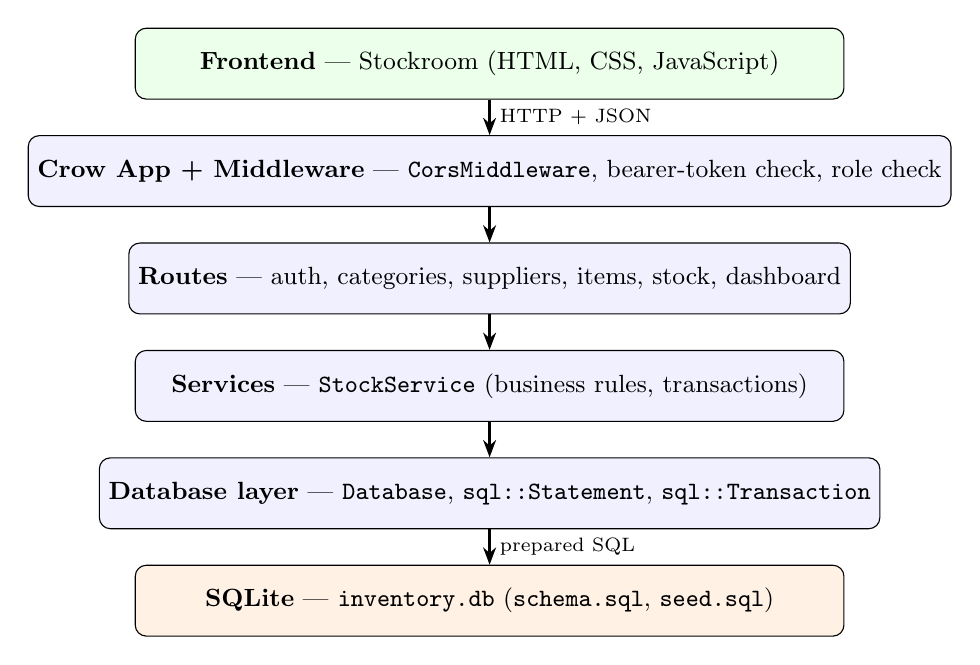
\begin{tikzpicture}[
  layer/.style={draw, rounded corners, fill=blue!6, minimum width=9cm, minimum height=0.9cm,
    font=\small, align=center},
  node distance=0.45cm]
  \node[layer, fill=green!8] (fe) {\textbf{Frontend} --- Stockroom (HTML, CSS, JavaScript)};
  \node[layer, below=of fe] (mw) {\textbf{Crow App + Middleware} --- \texttt{CorsMiddleware}, bearer-token check, role check};
  \node[layer, below=of mw] (rt) {\textbf{Routes} --- auth, categories, suppliers, items, stock, dashboard};
  \node[layer, below=of rt] (sv) {\textbf{Services} --- \texttt{StockService} (business rules, transactions)};
  \node[layer, below=of sv] (db) {\textbf{Database layer} --- \texttt{Database}, \texttt{sql::Statement}, \texttt{sql::Transaction}};
  \node[layer, below=of db, fill=orange!10] (sq) {\textbf{SQLite} --- \texttt{inventory.db} (\texttt{schema.sql}, \texttt{seed.sql})};
  \draw[flow] (fe) -- node[right, font=\scriptsize]{HTTP + JSON} (mw);
  \draw[flow] (mw) -- (rt);
  \draw[flow] (rt) -- (sv);
  \draw[flow] (sv) -- (db);
  \draw[flow] (db) -- node[right, font=\scriptsize]{prepared SQL} (sq);
\end{tikzpicture}
\end{document}
